\documentclass{standalone}
\usepackage{tikz}
\begin{document}
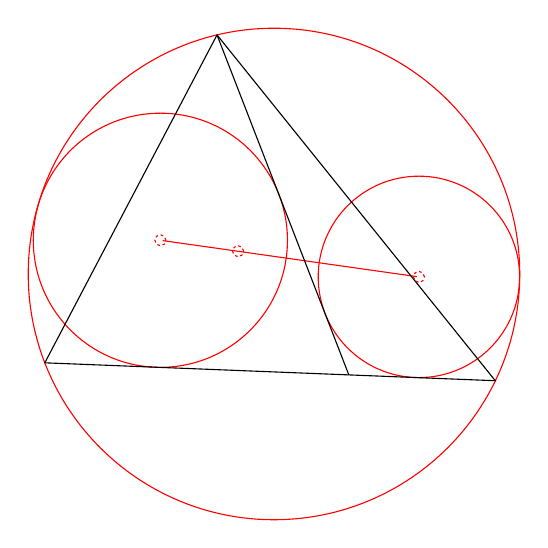
\begin{tikzpicture}[x=1pt,y=1pt]
\draw[red] (152.48,-135.15) circle (88.80);
\draw[red] (204.85,-136.20) circle (36.39);
\draw[red] (111.43,-122.97) circle (45.92);
\draw[red] (112.22,-123.08) -- (204.12,-136.11);
\draw (131.90,-48.77) -- (69.67,-167.25) -- (232.45,-173.72) -- cycle;
\draw (131.90,-48.77) -- (179.53,-171.62);
\draw[red, dash pattern=on 1pt] (204.85,-136.20) circle (2.00);
\draw[red, dash pattern=on 1pt] (139.51,-126.92) circle (2.00);
\draw[red, dash pattern=on 1pt] (111.44,-122.97) circle (2.00);
\end{tikzpicture}
\end{document}
